\documentclass[a4paper, openany]{memoir}

\usepackage[utf8]{inputenc}
\usepackage[T1]{fontenc} 
\usepackage[english]{babel}
\usepackage{amsmath}
\usepackage{amssymb}

\usepackage{booktabs}
\usepackage{fancyhdr}
\usepackage{float}
\usepackage{indentfirst}
\usepackage{graphicx}
\usepackage[linewidth=1pt]{mdframed}
\usepackage{multicol}
\usepackage{fancyvrb}

\pagestyle{fancy}
\fancyhf{}
\fancyhead[LE]{\leftmark}
\fancyhead[RO]{\rightmark}
\fancyhead[RE, LO]{PSD}
\fancyfoot[LE, RO]{\thepage}
\fancyfoot[RE, LO]{Pete Gautam}

\renewcommand{\headrulewidth}{1.5pt}

\chapterstyle{thatcher}
\setcounter{chapter}{11}

\begin{document}

\chapter{Evaluating Test Suites}
Testing a system requires effort. Even if test cases are automated, they still need to be developed and maintained. Each line of test case code should be considered as an ongoing cost for the development team, like maintaining a line of the application code.

The software team needs to be able to judge what investment they are likely to make on testing effort. The purpose of a test suite is to prevent the introduction of defects. There are properties we can consider for a test suite:
\begin{itemize}
    \item The effectiveness of a test suite. This is the ability of the test suite to prevent a defect being introduced to an application. Highly effective test suites ensure that the probability of a defect being introduction is very low. This is because there is a high probability that the defect will cause one or more test cases to fail.
    
    \item The efficiency of a test suite. This is the cost of maintaining the test suite. For a given set of defects prevented by a test suite, the fewer the lines of code/resources required to maintain the test suite, the more efficient it is.
\end{itemize}

In practice, the trade off between maintaining the test average and minimising the cost of conducting test per defect. This can be seen below.
\begin{figure}[H]
    \centering
    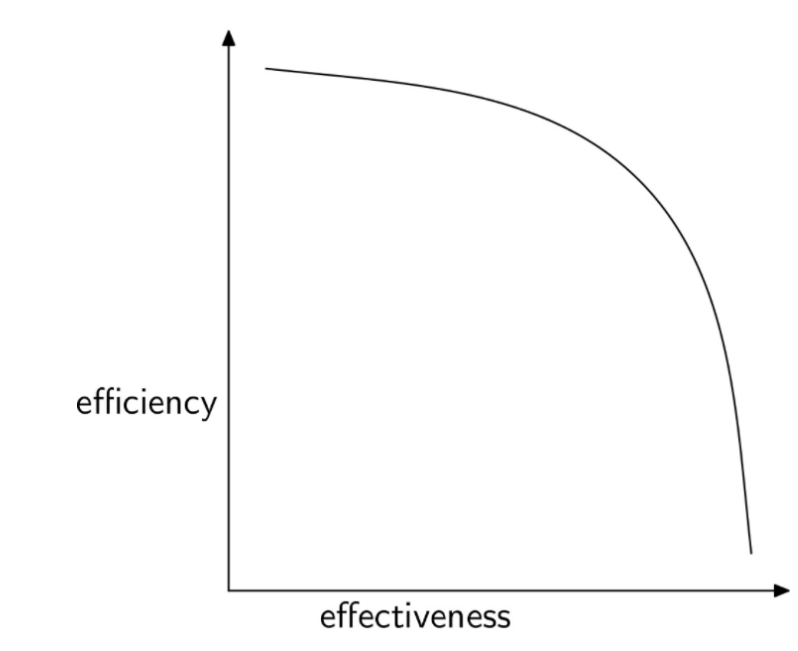
\includegraphics[scale=0.5]{src/12 Effectiveness v Efficiency.PNG}
    \caption{How effectiveness affects efficiency.}
\end{figure}
\noindent As the effectiveness increases, the cost of maintaining the test cases decreases. It is possible that some test cases are redundant, so we could remove them to increase effectiveness. On the other hand, we can also remove test cases. This will make it more efficient, but can lower coverage. In practice, the optimal efficiency and effectiveness lies somewhere in the middle. The software team needs to find a compromise between the effectiveness and the efficiency of test cases for a project.

\subsection{Measuring efficiency and effectiveness}
There are different useful metrics we use can use to measure the efficiency and effectiveness:
\begin{itemize}
    \item Post release reported defects. This is used to measure effectiveness of a test suite. If the number of user reported defects is low, then the test suite is effective at preventing defects.
    
    \item Lines of code (LoC) reached during test suite execution. If a test suite is able to exercise a high proportion of the code base, then it may be effective at uncovering defects in code base. Also, if there are fewer lines are executed by the test suite/defect, then it is more efficient the test suite.
    
    \item Test suite execution time. This measures efficiency, especially for unit test suites.
    
    \item Failed tests per defect. This is a useful measure of efficiency. If a large number of tests fail for a single defect, then the tests might be internally redundant.
    
    \item Test suite LoC. This is used to measure efficiency. The larger the code base, the less efficiency and costly the test suite is.
\end{itemize}

The table below shows these metrics in terms of efficiency and effectiveness.
\begin{table}[H]
    \centering
    \begin{tabular}{|l|c|c|}
        \hline
        Metric & Efficiency & Effectiveness \\
        \hline
        Post release reported defects & & \checkmark \\
        LoC reached during test suite execution & \checkmark & \checkmark \\
        Test suite execution time & \checkmark & \\
        Failed tests per defect & \checkmark & \\
        Test Suite LoC	& \checkmark  & \\
        \hline
    \end{tabular}
\end{table}

\subsection{Test suite runtime}
This is an efficiency metric. 
% A result of this is given below.
% \begin{figure}[H]
%     \centering
%     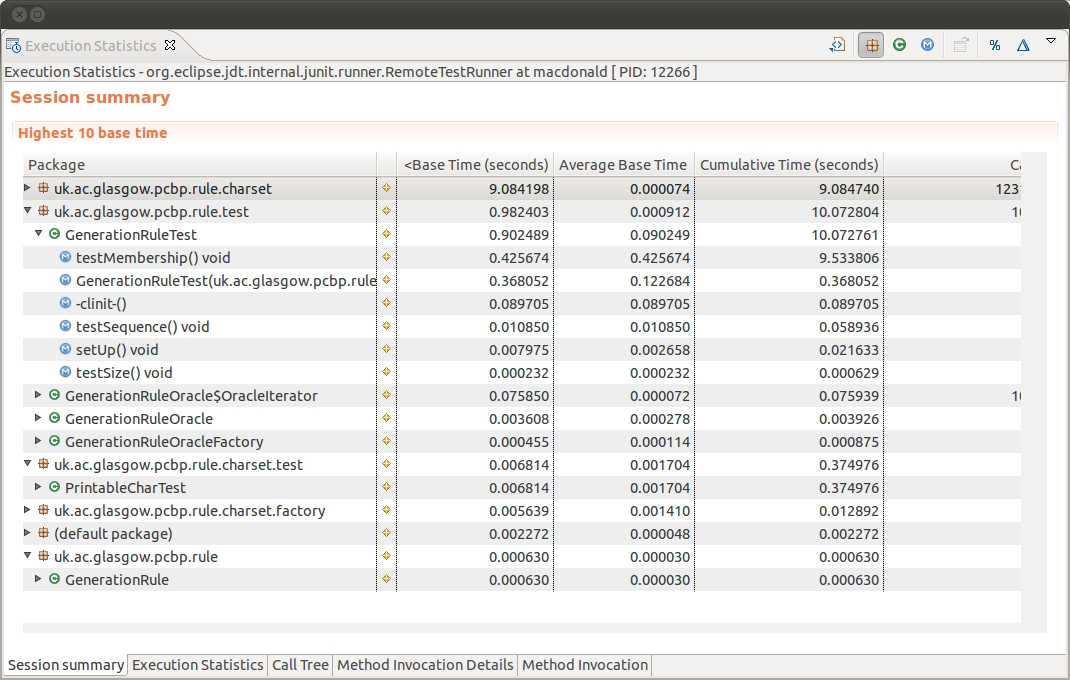
\includegraphics[scale=0.4]{src/12 test suite runtime.png}
%     \caption{Test suite runtime}
% \end{figure}
We expect unit tests to run quickly. Some researchers advocate for build time to be less than 10 minutes. This is usually acceptable for a build process but a test for a class/package should be executable within seconds. This allows the developer to incorporate them into the development workflow and ensure that they pass before changes to the module are committed to the change management system.

The (unit) test suites that take too long may fall into disuse. We can use tools such as profilers to evaluate the runtime of test suites and identify bottlenecks. The common cause of delays in test suites is the unit tests. This should be eliminated by using test doubles, e.g. mocks.

We can measure efficiency and efficiency using test suite runtime. We can track how different parts of the application are execution of test suite. It is often measured with lines of code (LoC), but it would be more precise if we use the statements executed or expressions evaluated. This is because not every line of code is evaluated within an execution.

Using LoC, we measure the effectiveness and efficiency using the following formulae:
\begin{align*}
    \text{effectiveness} &= \text{unique LoC executed}/\text{total LoC} \\
    \text{efficiency} &= \text{total LoC}/(\text{total LoC + LoC executed}).
\end{align*}
We can adjust these by ignoring some types of expressions, such as conditionals. Conditionals create different paths through the program, and might get evaluated more than once. Moreover, test code coverage is dynamic analysis (not static analysis). LoC can ignore 
\begin{itemize}
    \item import statements, 
    \item parentheses, 
    \item white space, 
    \item source code documentation, 
    \item uninteresting methods, such as getters/accessors and setters/mutators.
\end{itemize}

An example tool is given below.
\begin{figure}[H]
    \centering
    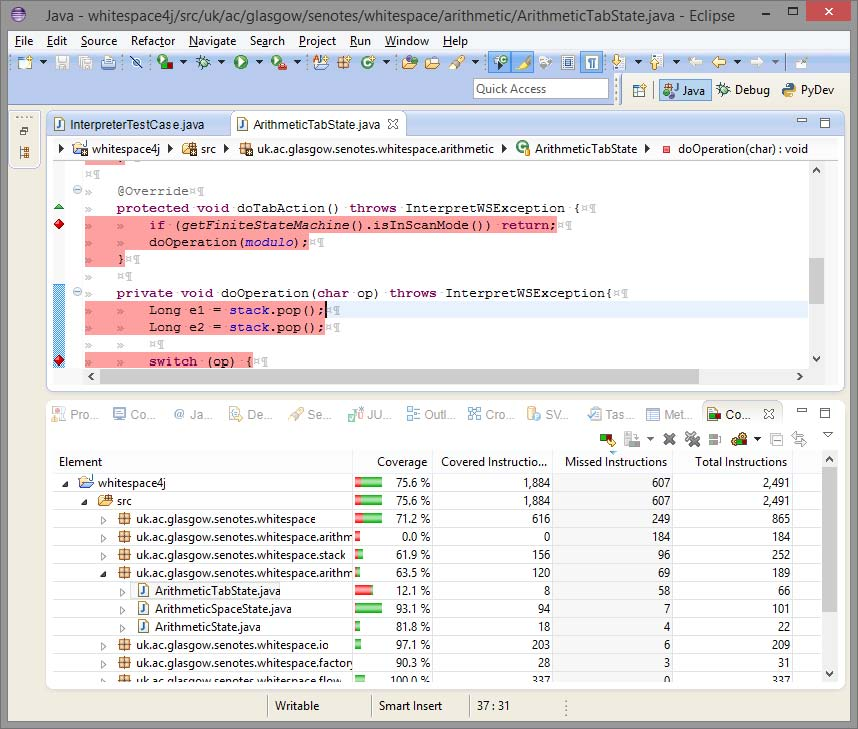
\includegraphics[scale=0.5]{src/12 Example tool.png}
    \caption{An example LoC code in Java}
\end{figure}
\noindent It is the execution of ECLEmma tool for calculating test code coverage. It is being used against whitespace programming language interpreter. There are many other similar tools, such as SonarCube.

There are many limits of test code coverage. Although it simple to implement, test code coverage can be misleading. This is because doesn't measure anything to do with defects. Also, test code coverage assumes that defects could be uniformly introduced into any line of code. 

Moreover, the test code coverage assumes that exercising a line of code, statement or expression is sufficient to expose any defects it might contain. This is not a safe assumption, and depends on the quality of the test suite. For example, consider the following example code in Python:
\begin{figure}[H]
    \centering
    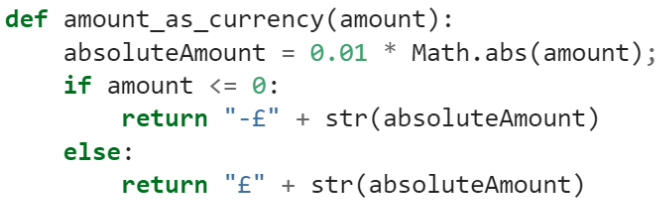
\includegraphics[scale=0.6]{src/12 Test coverage code.PNG}
    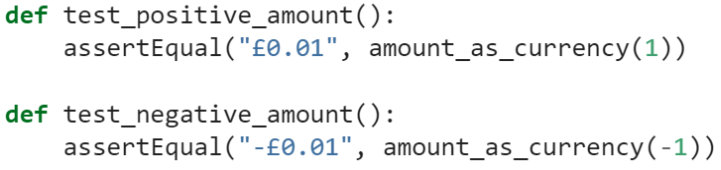
\includegraphics[scale=0.6]{src/12 Test coverage test.PNG}
\end{figure}
\noindent The two test cases achieve very high test coverage. All statements get executed and every expression is evaluated. However, the condition is still incorrect. If the value of \texttt{amount} is \texttt{0}, then it prints \texttt{-£0.00}. It can be corrected to \texttt{amount < 0} without breaking tests, which means that the test suite is underspecified.

A more common problem is to test coverage emphasised over defect coverage. Then, developers may be tempted to add tests to increase coverage, but lack assertions effectively gaining the metric.

\subsection{Mutation testing}
A more sophisticated measure of test suite effectiveness is the extent to which the test suite will detect the introduction of defects as a software system changes. This is called mutation testing. The aim of this technique is to estimate the likelihood that a change to the software system will be detected by one or more failing test cases. Tools for mutation testing include PiTest for Java, Mutpy for Python and Stryker for JS.

The technique works by representing the introduction of defects into a system as a combination of small-scale code mutations of the target system's code. The ability of the test case to act as a detection system for the presence of these mutations is analogous to its effectiveness in detecting the introduction of defects.

The key concept in mutation testing is a mutant. This is a mutation operator. We make small, legal changes to a program's logic that could affect its behaviour. Mutant operations are small and well-defined. They can be applied automatically in a wide variety of combinations to generate a large number of mutant programs. The mutant operations should always result in a viable mutant, i.e. syntax errors shouldn't be introduced in the source code.

We illustrate this with an example. The following is the source code.
\begin{figure}[H]
    \centering
    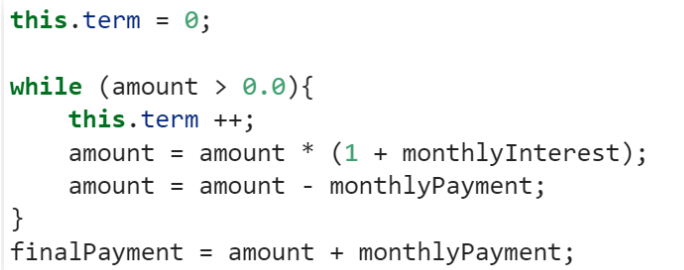
\includegraphics[scale=0.5]{src/12 Mutation 1.PNG}
\end{figure}
\noindent We can change the conditional operation, as given below.
\begin{figure}[H]
    \centering
    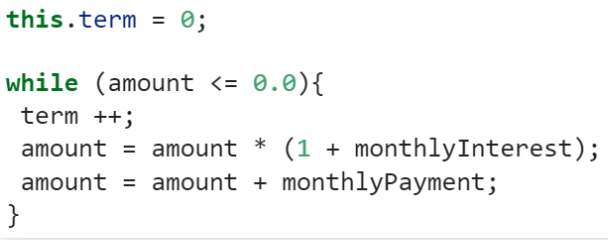
\includegraphics[scale=0.5]{src/12 Mutation 2.PNG}
\end{figure}
\noindent We can replace infix mathematical operator with another one.
\begin{figure}[H]
    \centering
    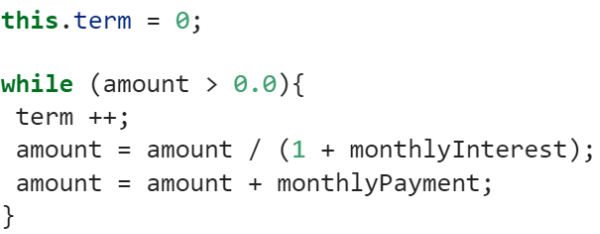
\includegraphics[scale=0.5]{src/12 Mutation 3.PNG}
\end{figure}
\noindent We can also replace increments with decrementors.
\begin{figure}[H]
    \centering
    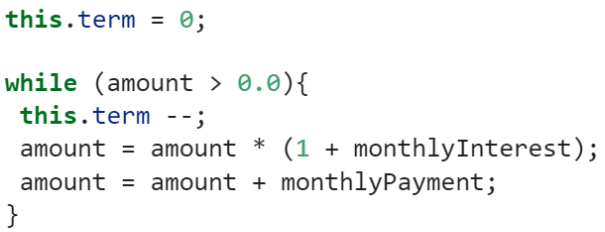
\includegraphics[scale=0.5]{src/12 Mutation 4.PNG}
\end{figure}

There are many types of mutation operations, such as:
\begin{itemize}
    \item replacing conditional operations with their boundary counterparts;
    \item replacing infix mathematical operators with other operations;
    \item replacing member field values with default/other values (e.g. replacing an integer with 0);
    \item replacing variable values with default values;
    \item replacing constructor calls with null assignments;
    \item replacing returned values with default values;
    \item replacing method call results with default values.
\end{itemize}

The following diagram illustrates the mutation testing process.
\begin{figure}[H]
    \centering
    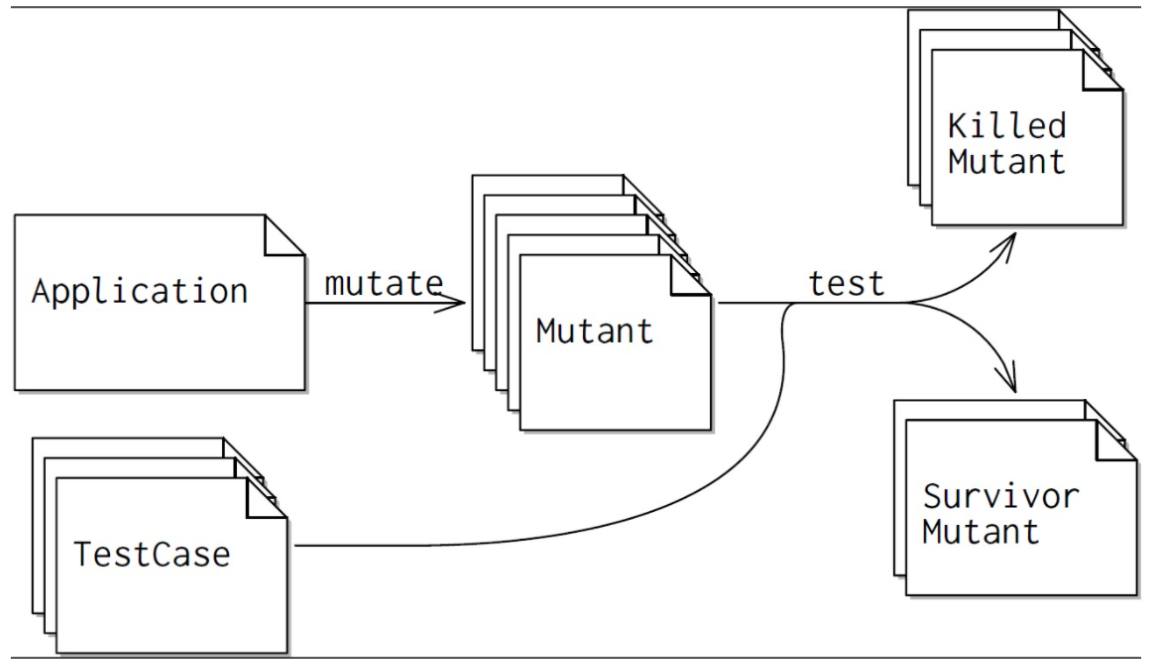
\includegraphics[scale=0.35]{src/12 Mutation testing workflow.PNG}
    \caption{The mutation testing process}
\end{figure}
\noindent We start with the baseline version of the software and the test cases. We refer to the baseline version as the green version. This is because we expect the baseline version to pass all the test cases in the suite; it should be free of defects.

We then create a large number of mutants by applying random combination of mutant operators to the system's code. This is applied to the system's source code, binaries or any other intermediates, as appropriate. 

Next, the test suite is applied to each of the application in turn and each outcome of the test is categorised. A killed mutant is one that was successfully detected by the test suite. A survivor mutant is one that successfully passed the test suite. This can indicate that some aspect of logic was not covered by a test. However, it is also possible for the mutant to be essentially the same as the baseline code. We need to evaluate each survivor mutant manually to check if we can improve the test code. An undetermined mutant is one where we encountered a runtime error or the timeout threshold was breached.

Once all the mutants are tested, we can calculate the metrics for effectiveness and efficiency. Effectiveness is given by the mutant survival rate, where
\[\text{mutant survival rate} = \# \text{survivors}/\text{total mutants}.\]
A lower survival rate means that the test suite is more effective. The efficiency is given by
\[\text{efficiency} = \# \text{killed mutants}/\# \text{failed tests}.\]
Ideally, there should be 1-to-1 relationship between killed mutants and failed tests. If one mutant causes a large number of test cases to fail, then it is possible that the test cases overlap. This needs to be considered carefully since it depends on how the mutants are generated. For example, we might have a large number of very similar mutations, which might mean that it isn't diverse enough to give a proper indication of the efficiency of the test suite.

A disadvantage of this approach is that it does not address the converse issue of redundancy. That is, we could have a set of similar tests that never fail, and we would still need to maintain them. An alternative approach is to try to minimise the number of test cases. For a given set of mutants, this is the smallest number of test cases that can cover all the defects. Finding this set is hard, so tools that provide this feature usually do so by approximating it.

The following table shows a test case result.
\begin{table}[H]
    \centering
    \begin{tabular}{|c|c|c|c|c|c|}
        \hline
        & \multicolumn{2}{c|}{lines} & \multicolumn{2}{c|}{mutants} \\
        \hline
        Artifact & covered & total & killed & total \\
        \hline
        Mortgage & 7 & 8 & 3 & 4 \\
        RepaymentPlanImpl & 27 & 28 & 25 & 27 \\
        uk.ac.glasgow.senotes.bank & 34 & 36 & 28 & 31 \\
        \hline
    \end{tabular}
\end{table}
\noindent We are running PiTest against 4 test cases. The application is quite small, so a high proportion of mutants are killed by the test cases. We can compare test code coverage of lines as well.

The graph below show how the number of killed mutant changes as we use fewer test cases:
\begin{figure}[H]
    \centering
    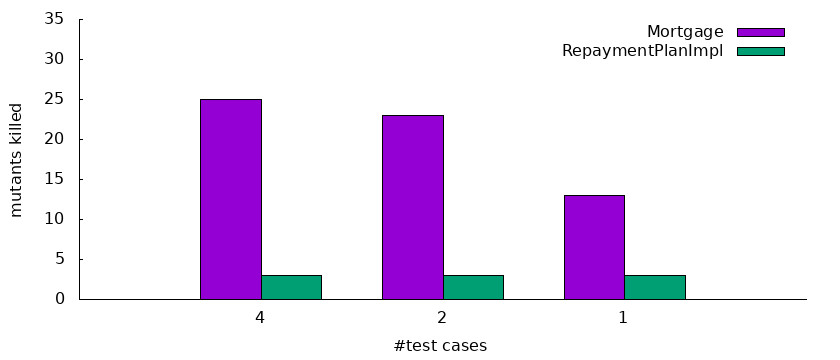
\includegraphics[scale=0.5]{src/12 Efficiency v no of test cases.png}
    \caption{The number of killed mutants as the number of test cases changes.}
\end{figure}
\noindent Using this graph we can decide whether to remove some test cases to improve efficiency. The graph shows that removing 2 of the 4 test cases barely lowers the number of mutants killed, but removing an extra test case dramatically lowers the number of mutants killed. This suggests that the team should keep the two most effective test cases in the test suite. We will need to review this decision periodically as the target application and the test suite evolves.

\subsection{Configuration space and optimising mutation testing}
The metrics produced by mutation testing depend on a range of configuration options, such as:
\begin{itemize}
    \item the choice of mutation operations- this impacts the types of defects simulated by the system, e.g. conditional mutant operation can simulate an off by 1 error.
    \item the number and the combination of mutations applied to a program- the more the mutants created, the richer the set of defects and the better the test case suite. However, we are more likely to have redundant mutants.
    \item the timeout period for completing a test case- this affects the number of undetermined mutants. It isn't possible to determine which mutants will terminate by the Halting problem. So, we need to set a timeout for each test. However, this is typically the same as the original program. It is possible that this is not enough time for mutants, e.g. if they run a loop for more cycles than the normal program.
    \item the scope of the test suite for each mutant- it can be more useful to limit the selection of test cases that need to be applied to a mutation. For example, PiTest determines the coverage of each test before undertaking mutation testing. This can be useful in selecting the test cases that need to be applied to a mutant and helps to avoid running tests whose scope hasn't changed since the previous run. However, there is a risk if the test suite has low coverage. In that case, introducing mutants might reach other parts of the program that aren't reached during the green test phase. 
\end{itemize}

\subsection{Comparing mutation test results}
We need to be wary when comparing mutation test results across projects. Mutation tools take into account the nature of target application. For instance, two different configurations for different projects will have different effects on the performance of the underlying test suite. Moreover, two projects may have very different characteristics that are better tested using very different configurations, e.g. comparing system design for interactive use with that of volume batch processing of scientific calculations.

\subsection{Limitations of mutation testing}
Although mutation testing is better than test code coverage, it has limitations. The effectiveness of the mutation testing process is dependent on careful configuration of the process. Even with careful configuration, mutation operations (or their combination) may not be representative of the types of defects that are introduced in a project. For example, precision defects may not be manifested by mathematical mutations, and external dependency defects may not be captured if the test suite uses mocks. 

Moreover, mutation testing takes a long time to run because the entire test suite must be executed on each mutant. There are some optimisations available to mitigate this, but it is often better to run mutation testing as a nightly build process rather than performing it on every commit of the project. This is partly because we don't expect the characteristics of mutation testing to change drastically between each commit.

In summary, evaluating test suites is an important component of the quality assurance process.

\end{document}